\chapter{Implementace}
\label{ch:implementation}
Tato sekce obsahuje popis implementace aplikace, která byla vytvořena na základě analýzy v předchozích kapitolách. V této sekci se zaměřím na popis jednotlivých komponent aplikace, které byly vytvořeny a následně nasazeny do produkce. Dále se zaměřím na popis týmové spolupráce, která byla nutná pro vytvoření celého projektu, a na závěr se zaměřím na popis problémů, které se v průběhu vývoje objevily.

\section{Požadavky na implementaci}
\label{sec:implementation-requirements}
Požadavků na implementaci ze strany administrativního rozhraní není mnoho, přesto ale existují. V této sekci se pokusím popsat veškeré požadavky, které byly kladeny na implementaci aplikace během jejího návrhu.

Během vývoje se tyto požadavky průběžně měnily, proto je celkem obtížné vždy předem definovat úplný seznam požadavků.

\subsection*{Funkční požadavky}
\label{subsec:implementation-requirements-functional}

\begin{description}
    \item \textbf{Přihlášení} -- Jelikož se jedná o aplikaci administrační, vstup do aplikace je možný pouze pro přihlášené uživatele. Z funkčního hlediska je v rámci projektu využita pouhá role \textit{Administrátora}, z toho důvodu není nutné rozlišovat mezi různými uživatelskými rolemi.
    \item \textbf{Správa obsahu} -- Hlavním účelem tohoto rozhraní je správa obsahu hry, bez možnosti formulářové editace obsahu jsou administrátoři omezeni na surovou správu dat pomocí editace záznamů v databázi nebo změnou výchozích dat v souborech. Z tohoto důvodu je nutné zajistit plnou možnost správy obsahu hry stylem \textit{CRUD}.
    \item \textbf{Filtrace a vyhledávání} -- Pro přehlednou správu dat jednotlivých tabulek je důležité umožnit administrátorům rychlé a efektivní prvky filtrování.
    \item \textbf{Vykreslování} -- Určité části projektu obsahují grafické prvky, které je pro lepší pochopení nutné graficky zpracovat a vykreslit na obrazovku. Pro tento účel bude využit HTML prvek \textit{canvas}, který umožňuje grafické vykreslování.
    \item \textbf{Validace} -- Při vkládání obsahu do databáze pomocí API je nutné klást důraz na správné formátování všech dat před odesláním.
    \item \textbf{Export} -- Pro úspěšné zálohování dat je nutné umožnit export všech dat do souboru, který bude následně kompatibilní s automatickým importem do databáze.
\end{description}

\section{Komponenty aplikace}
\label{sec:implementation-components}
V případě implementace administračního rozhraní nelze pouze implementovat frontend aplikace, ale je nutné implementovat i backend, který zajišťuje zpracování dat, a jejich následnou komunikace s API\@.

V níže uvedených sekcích se blíže zaměřím na implementaci jednotlivých komponent.

\subsection{Frontend}
\label{subsec:implementation-frontend}
Vývoj frontendu byl zahájen vyhledáním již předem vytvořené šablony a to z důvodu usnadnění designových potřeb a možnosti se plně věnovat další části aplikace. Výsledek hledání byl úspěšný a nalezená šablona byla kompatibilní s frameworkem Django. Přesněji se jedná o šablonu od autora \textit{Themesberg}\footnote{\href{https://themesberg.com/}{https://themesberg.com/}}, konkrétně šablona administračního rozhraní \textit{Volt}\footnote{\href{https://themesberg.com/product/django/volt-admin-dashboard-template}{https://themesberg.com/product/django/volt-admin-dashboard-template}}.

Po úspěšné instalaci bylo dalším krokem rozvržení navigace, která se nachází na levé straně stránky. Jednotlivé odkazy následně směřují na podstránky, kde lze vidět obsah jednotlivých tabulek, ve kterých se nachází možnost filtrovat, hledat nebo provádět zbytek CRUD operací.

Průběh otevření každé ze stránek navigace je možné vidět na Diagramu~\ref{fig:OpenPage}, kde prvně dochází k ověření přihlášení uživatele, následnému zobrazení dočasného obsahu stránky, který je v pozdější době asynchronně doplněn obsahem z API\@.

\processDiagram{diagrams/OpenPage}{OpenPage}{0.75\textwidth}{Diagram zobrazující otevření stránky}

\subsection{Backend}
\label{subsec:implementation-backend}
Backend aplikace, vytvořen pod frameworkem Django stejně jako část frontendu, zajišťuje zpracování dat podle žádosti uživatele. K získání dotazu dochází pomocí URL adresy, která je v aplikaci zpracována pomocí \textit{view} komponenty pod následnou routing adresou. Po vyřízení požadavku jsou data zpět odeslána uživateli, který je následně upozorněn na úspěšné provedení akce.

Níže zobrazený Diagram~\ref{fig:NewObject} popisuje průběh vytvoření nebo editace objektu, kde tato funkcionalita reprezentuje nejdůležitější prvek celé aplikace z důvodu, že umožňuje definovat herní obsah. Po odeslání formuláře dochází ke kontaktování API, která následně požadavek zpracuje a odešle zpět odpověď, jež je následně zobrazena uživateli.

\processDiagram{diagrams/NewObject}{NewObject}{0.75\textwidth}{Diagram reprezentující průběh vytvoření nebo editace objektu}

\subsection{API}
\label{subsec:implementation-api}
Přestože API je součástí práce kolegy, pro usnadnění a zabezpečení jsem použil vlastní lokální API, které zpracovává dotazy, a v případě, že je nutné získat data, odešle požadovaný dotaz směrem na veřejné API pod url adresou \textit{https://api.tts-game.fun}. Díky zmíněnému mezikroku je možné zabezpečit identitu API klíče, který zůstává skrytý pod lokálním API spravovaným jazykem Python. V opačném případě by tento klíč byl odesílán s každým dotazem, čímž by se stal zachytitelný pro útočníky.

V našem případě jsme použili pro autorizaci obyčejný token, které je uložen v nastavení API. Nejedná se o nejbezpečnější použití, ale z pohledu této práce je dostatečné. Schéma komunikace při použití prostřední API je možné vidět na Obrázku~\ref{fig:api_communication}.

\begin{figure}[H]
    \centering
    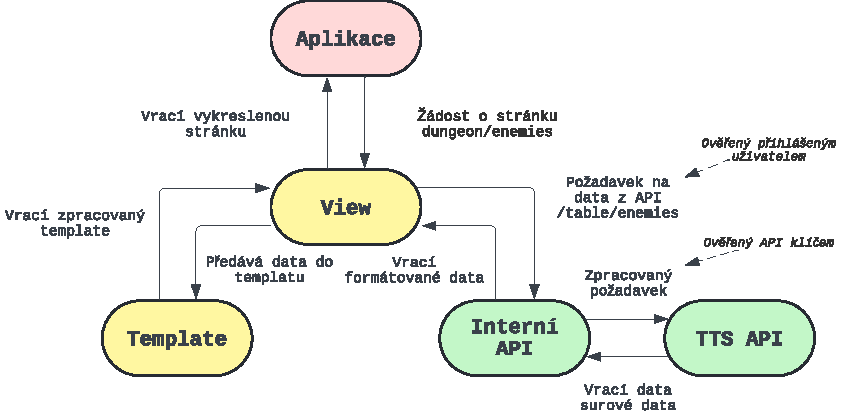
\includegraphics[width=0.96\textwidth]{diagrams/API_Communication}
    \caption{Schéma komunikace mezi jednotlivými komponentami}
    \label{fig:api_communication}
\end{figure}

Níže ve zdrojovém kódu~\ref{lst:api-cross-processing-api},~\ref{lst:api-cross-processing} lze vidět kus zdrojového kódu který se tak stará o mapování interního API a následného zpracování požadavku. Pomocí urlpatterns dochází k namapování poždavku, které je následně poslán do backendu djanga. Kde dojde k zpracování a případné zaslání dotazu na veřejné API\@.

Na řádku 14 zdrojového kódu~\ref{lst:api-cross-processing-api} lze vidět šifrování administrátorského jména a hesla do tokenu, který je následně na řádku 24 přidáván jako autorizace do veřejného API.
\pagebreak

\lstinputlisting[language=Python, caption={Zpracování interního API v pythonu}, label={lst:api-cross-processing-api}]{sourceCodes/djangoAPI.py}
\lstinputlisting[language=Python, caption={Zpracování interního API v pythonu}, label={lst:api-cross-processing}]{sourceCodes/djangoRequestAPI.py}

\section{Volba technologií}
\label{sec:implementation-technologies}
V této sekci se budu věnovat výběru technologií, které jsem zvolil v průběhu implementace aplikace. Výběr technologií většinou vychází z analýzy uvedené v Kapitole~\ref{ch:theory_and_analysis} nebo z osobních zkušeností, které jsem získal v průběhu studia.

\subsection{Framework}
\label{subsec:implementation-technologies-framework}
Jak bylo zmíněno v sekci analýze rozhraní, pro vývoj aplikace administrativního rozhraní jsem zvolil framework Django. Díky tomuto frameworku jsem mohl využít jeho širokou škálu již předem zakomponovaných funkcí, které mi usnadnily vývoj. Díky těmto funkcím jsem se mohl zaměřit na vývoj samotného rozhraní, které jsem psal v jazyce TypeScript s využitím frontendového frameworku Bootstrap.

Framework jako samotný neobsahuje rozšířené prvky pro použití na frontendu, z toho důvodu jsem byl nucen psát si tyto komponenty sám. Pro jejich vývoj jsem využil jazyk TypeScript, kde jsou výsledné komponenty mezi stránkami sdíleny. Pro dynamické načítaní obsahu je využíváno asynchronní načítání dat pomocí AJAXu po prvotním načtení stránky a po jeho zpracování dojde k překreslení části stránky.

Jedna z komponent, která slouží pro asynchronní získávání dat je zobrazena v ukázce Zdrojového Kódu~\ref{lst:data-request-component}. Tato komponenta slouží pro nahrazení dočasného obsahu na stránce daty, která jsou získána v pozdějším procesu pomocí XMLHttpRequestu, který je volán na interní API, kde následně dochází k vyplnění obsahu templatu daty a jeho zobrazení.

\pagebreak
\lstinputlisting[language=TypeScript, caption={Komponenta pro získání asynchronních dat}, label={lst:data-request-component}]{sourceCodes/DataRequestComponent.ts}

\subsection{Knihovny}
\label{subsec:implementation-technologies-libraries}
Při vývoji aplikace jsem využil několik knihoven třetích stran, které mi usnadnily vývoj a zároveň zrychlily proces vývoje, protože nebylo nutné psát vše od základu. Mezi tyto knihovny patří:

\begin{description}
    \item \textbf{Font Awesome}\footnote{\href{https://fontawesome.com/}{https://fontawesome.com/}} je knihovna ikon, která disponuje širokou škálou veřejně dostupných ikon, které jsou zdarma k použití. Ve vývoji jsem tyto ikony použil pro reprezentaci různých akcí, které může uživatel provést.
    \item \textbf{Bootstrap}\footnote{\href{https://getbootstrap.com/}{https://getbootstrap.com/}} jsem použil jako frontendovou knihovnu předem napsaných stylů, díky kterým jsem mohl rychle vytvořit efektivní a responzivní rozhraní. Bootstrap nabízí širokou škálu komponent, které jsou podrobně popsány v dokumentaci.
    \item \textbf{SweetAlert2}\footnote{\href{https://sweetalert2.github.io/}{https://sweetalert2.github.io/}} je knihovna, která umožňuje jednoduše zobrazovat notifikace a upozornění uživateli. Knihovna byla využita například pro zobrazení upozornění při chybě nebo úspěšném provedení akce.
    \item \textbf{GoJS}\footnote{\href{https://gojs.net/latest/index.html}{https://gojs.net/latest/index.html}} obsahuje funkce pro jednoduché a efektivní vytváření grafů, které byly využity pro interaktivní zobrazení návaznosti lokací v rámci kampaně.
    \item \textbf{Animate.css}\footnote{\href{https://animate.style/}{https://animate.style/}}, Hover.css\footnote{\href{https://ianlunn.github.io/Hover/}{https://ianlunn.github.io/Hover/}} je knihovna, která obsahuje předpřipravené animační styly, které stačí pouze aplikovat pomocí CSS tříd nebo dynamicky pomocí JavaScriptu.
    \item \textbf{Notiflix}\footnote{\href{https://notiflix.github.io/}{https://notiflix.github.io/}} je další z knihoven pro zobrazování notifikace, v tomto projektu jsem ale pro notifikace zvolil knihovnu SweetAlert2. Z toho důvodu je tato knihovna využita pouze pro blokaci uživatelského vstupu během načítání nebo zpracování dat formou loading spinneru.
    \item \textbf{NoUISlider}\footnote{\href{https://refreshless.com/nouislider/}{https://refreshless.com/nouislider/}} je knihovna, která do prvků HTML přidává možnost vytvořit posuvníky, které je následně možné využit pro výběr hodnoty z rozsahu. Příklad jeho použití je ve formuláři s filtrací dat.
\end{description}

\subsection{Jazykový procesor}
\label{subsec:implementation-technologies-compiler}
Výběr jazyka pro uživatelské rozhraní je důležitým aspektem v případě aplikací určených pro širokou veřejnost. V rámci této práce byl jako primární jazyk rozhraní zvolen jazyk anglický, což je nejuniverzálnější jazyk na světě, díky čemuž je aplikace přístupná širokému spektru uživatelů bez potřeby překladu. Nicméně pro některé uživatele může být angličtina obtížná, a z toho důvodu byl implementován jazykový procesor, který umožňuje integraci více jazyků do aplikace.

Pro podporu vícejazyčné funkčnosti byla v této práci využita knihovna i18next\footnote{\href{https://www.i18next.com/}{https://www.i18next.com/}}, která je jednou z nejrozšířenějších nástrojů pro lokalizaci. Tato knihovna automaticky zpracovává jazykové soubory a aplikuje odpovídající překlady v závislosti na nastavení uživatele. Tímto způsobem je pro vývojáře snadné nastavit výchozí jazyk a později přidat další překlady.

\lstinputlisting[language=JavaScript, caption={Ukázka využití knihovny i18next}, label={lst:i18next-example}]{sourceCodes/LanguageLocalization.js}

Na ukázce Zdrojového Kódu~\ref{lst:i18next-example} je zobrazeno využití knihovny v případě obyčejného použití v JavaScriptu. Knihovna sama o sobě nabízí možnou integraci do různých frameworků jako například použitý freamework Django v této práci.

\subsection{Autorizace}
\label{subsec:implementation-technologies-authorization}
Autorizace do administračního rozhraní zajišťuje backend aplikace, konkrétně tedy Django, které tuto funkcionalitu zajišťuje pomocí vlastního systému autorizace. Konkrétně se aplikace pro zabezpečení nazývá \textit{django.contrib.auth}, jedná se tak o balíček v rámci frameworku Django. Pro přihlášení do aplikace je nutné zadat uživatelské jméno a heslo do formuláře na přihlašovací stránce, po odeslání formuláře dochází k ověření uživatele pomocí interní databáze. V případě úspěchu je uživatel také uložen do session, která se následně stará o udržení přihlášení a ověření uživatele při každém požadavku.

Na ukázce Zdrojového Kódu~\ref{lst:djangoViewURL} je možné vidět dekorátor \textit{@login\_required}, která zajišťuje, že uživatel je přihlášen a má tak přístup k danému view. V případě, že uživatel není přihlášen, dojde k přesměrování na přihlašovací stránku.

\lstinputlisting[language=Python, caption={Ukázka zpracování požadavku Djangem při ověření}, label={lst:djangoViewURL}]{sourceCodes/djangoView.py}

\subsection{Vyhledávání a filtrování}
\label{subsec:implementation-technologies-search}
Vyhledání a filtrování jsem implementoval pomocí funkce \textit{search} a \textit{filter}, které jsou zahrnuty v rámci API rozhraní. Pomocí těchto funkcí je tak možné přijmout z uživatelského rozhraní dotaz pomocí textového pole a následně dotaz odeslat na API. Po zpracování dotazu je odpověd od API znovu vykreslena do tabulky, tentokrát již pouze s vyfiltrovanými daty.

Filtrace dat funguje stejným způsobem, kde pomocí vytvořeného modálního okna lze zadat přesné hodnoty, které se mají zobrazit. Po odeslání dotazu je následně zobrazen pouze obsah, který odpovídá zadaným hodnotám.

\subsection{Validace dat}
\label{subsec:implementation-technologies-validation}
Validace dat, která je v rámci aplikace prováděna, je zajištěna opět na straně API. Kde v každém formuláři dochází k okamžité validaci pomocí zaslání dat formuláře na API endpoint určený pro daný objekt. V případě, že data nejsou správná, uživatel dostává okamžitě zpětnou vazbu, formou notifikace, která jednoduše informuje o chybě, kterou tak lze následně urychleně opravit.

Tento způsob kontroly tak zajišťuje stabilní a korektní data v databázi a zároveň zabraňuje vzniku chyb, které by mohly být způsobeny nesprávnými daty. Proces validace dat je zobrazen na Diagramu~\ref{fig:NewObject}, kde dochází ke komunikaci s API\@.

\subsection{Databáze}
\label{subsec:implementation-technologies-database}
Pro ukládání dat v našem systému jsme zvolili databázi MariaDB\footnote{\href{https://mariadb.org/}{https://mariadb.org/}}, která nám byla doporučena vedoucím práce. Nejedná se o nejmodernější databázi, ale disponuje vysokou stabilitou a širokou historii použití. Databázi jsme pro bezpečnější použití rozdělili na dvě \textit{tts\_api} a \textit{tts\_api\_dev}, kde první obsahuje základní data a druhá data testovací. Pro vytvoření databáze byly následně využity skripty, které budou dále popsány v sekci Automatizace.

\subsubsection*{Schéma}
\label{subsubsec:implementation-technologies-database-scheme}
Schéma databáze bylo vytvořeno placeným softwarem DbDiagram.io\footnote{\href{https://dbdiagram.io/home}{https://dbdiagram.io/home}}, který nabízí možnost živého návrhu schématu, na kterém se tak mohl podílet každý člen týmu zároveň, což usnadnilo aktivní vývoj. Zkrácené schéma o M:N relacích je zobrazeno na Obrázku~\ref{fig:db_scheme}. Software DbDiagram nabízí možnost exportu schématu do různých formátů, které byly následně využity pro vytvoření databáze v MariaDB\@.

\subsubsection*{Automatizace}
\label{subsubsec:implementation-technologies-database-automatization}
Automatizace vytváření a plnění databáze je důležitá pro kontinuální vývoj softwaru a v praxi se nazývá \textit{migrace}. Skripty pro vytvoření a naplnění databáze byly napsány v skriptovacím jazyce Python\footnote{\href{https://www.python.org/}{https://www.python.org/}}. Tyto skripty byly vytvořeny tak, aby při jejich spuštění provedly kompletní smazání databáze, následně pak její znovuvytvoření a pozdější naplnění. Ukázka výstupu vytvořených skriptů je zobrazena v příloze~\ref{fig:databaseScriptsOutput}.

Pro vytvoření databáze byl použit SQL soubor, který se po každé úpravě v nástroji DbDiagram.io vyexportoval. Jakmile byla databáze resetována do výchozí podoby a vše proběhlo úspěšně, došlo na řadu její plnění, pro které jsou data uložena v souborech ve formátu JSON. Tyto soubory lze jednoduše exportovat z administračního rozhraní a uložit pro pozdější použití při obnově nebo plnění databáze.

Plnění databáze ale není jednoduchý proces, neboť je nutné zajistit správné pořadí cizích klíčů, bez kterého se žádná tabulka nemůže bezchybně naplnit. Pro tento účel byl vytvořen diagram reprezentující abstraktní schéma databáze s prioritou jednotlivých tabulek, který je zobrazen na Obrázku~\ref{fig:db_table_priority}. Tento diagram slouží jako návod pro správné nastavení priorit jednotlivých tabulek.

Pro čtení priority z Grafu~\ref{fig:db_table_priority} je nutné vždy začít od dané tabulky a spočítat nejhlubší cestu k nejvzdálenější tabulce proti směru šipek. Tabulky s největší prioritou mají k sobě největší počet cest. V případě, že tabulka k sobě nemá žádnou cestu, je její priorita automaticky nastavena na 1. Tabulka priority je následně zobrazena v Tabulce~\ref{tab:db_table_priority}.

\begin{figure}[H]
    \centering
    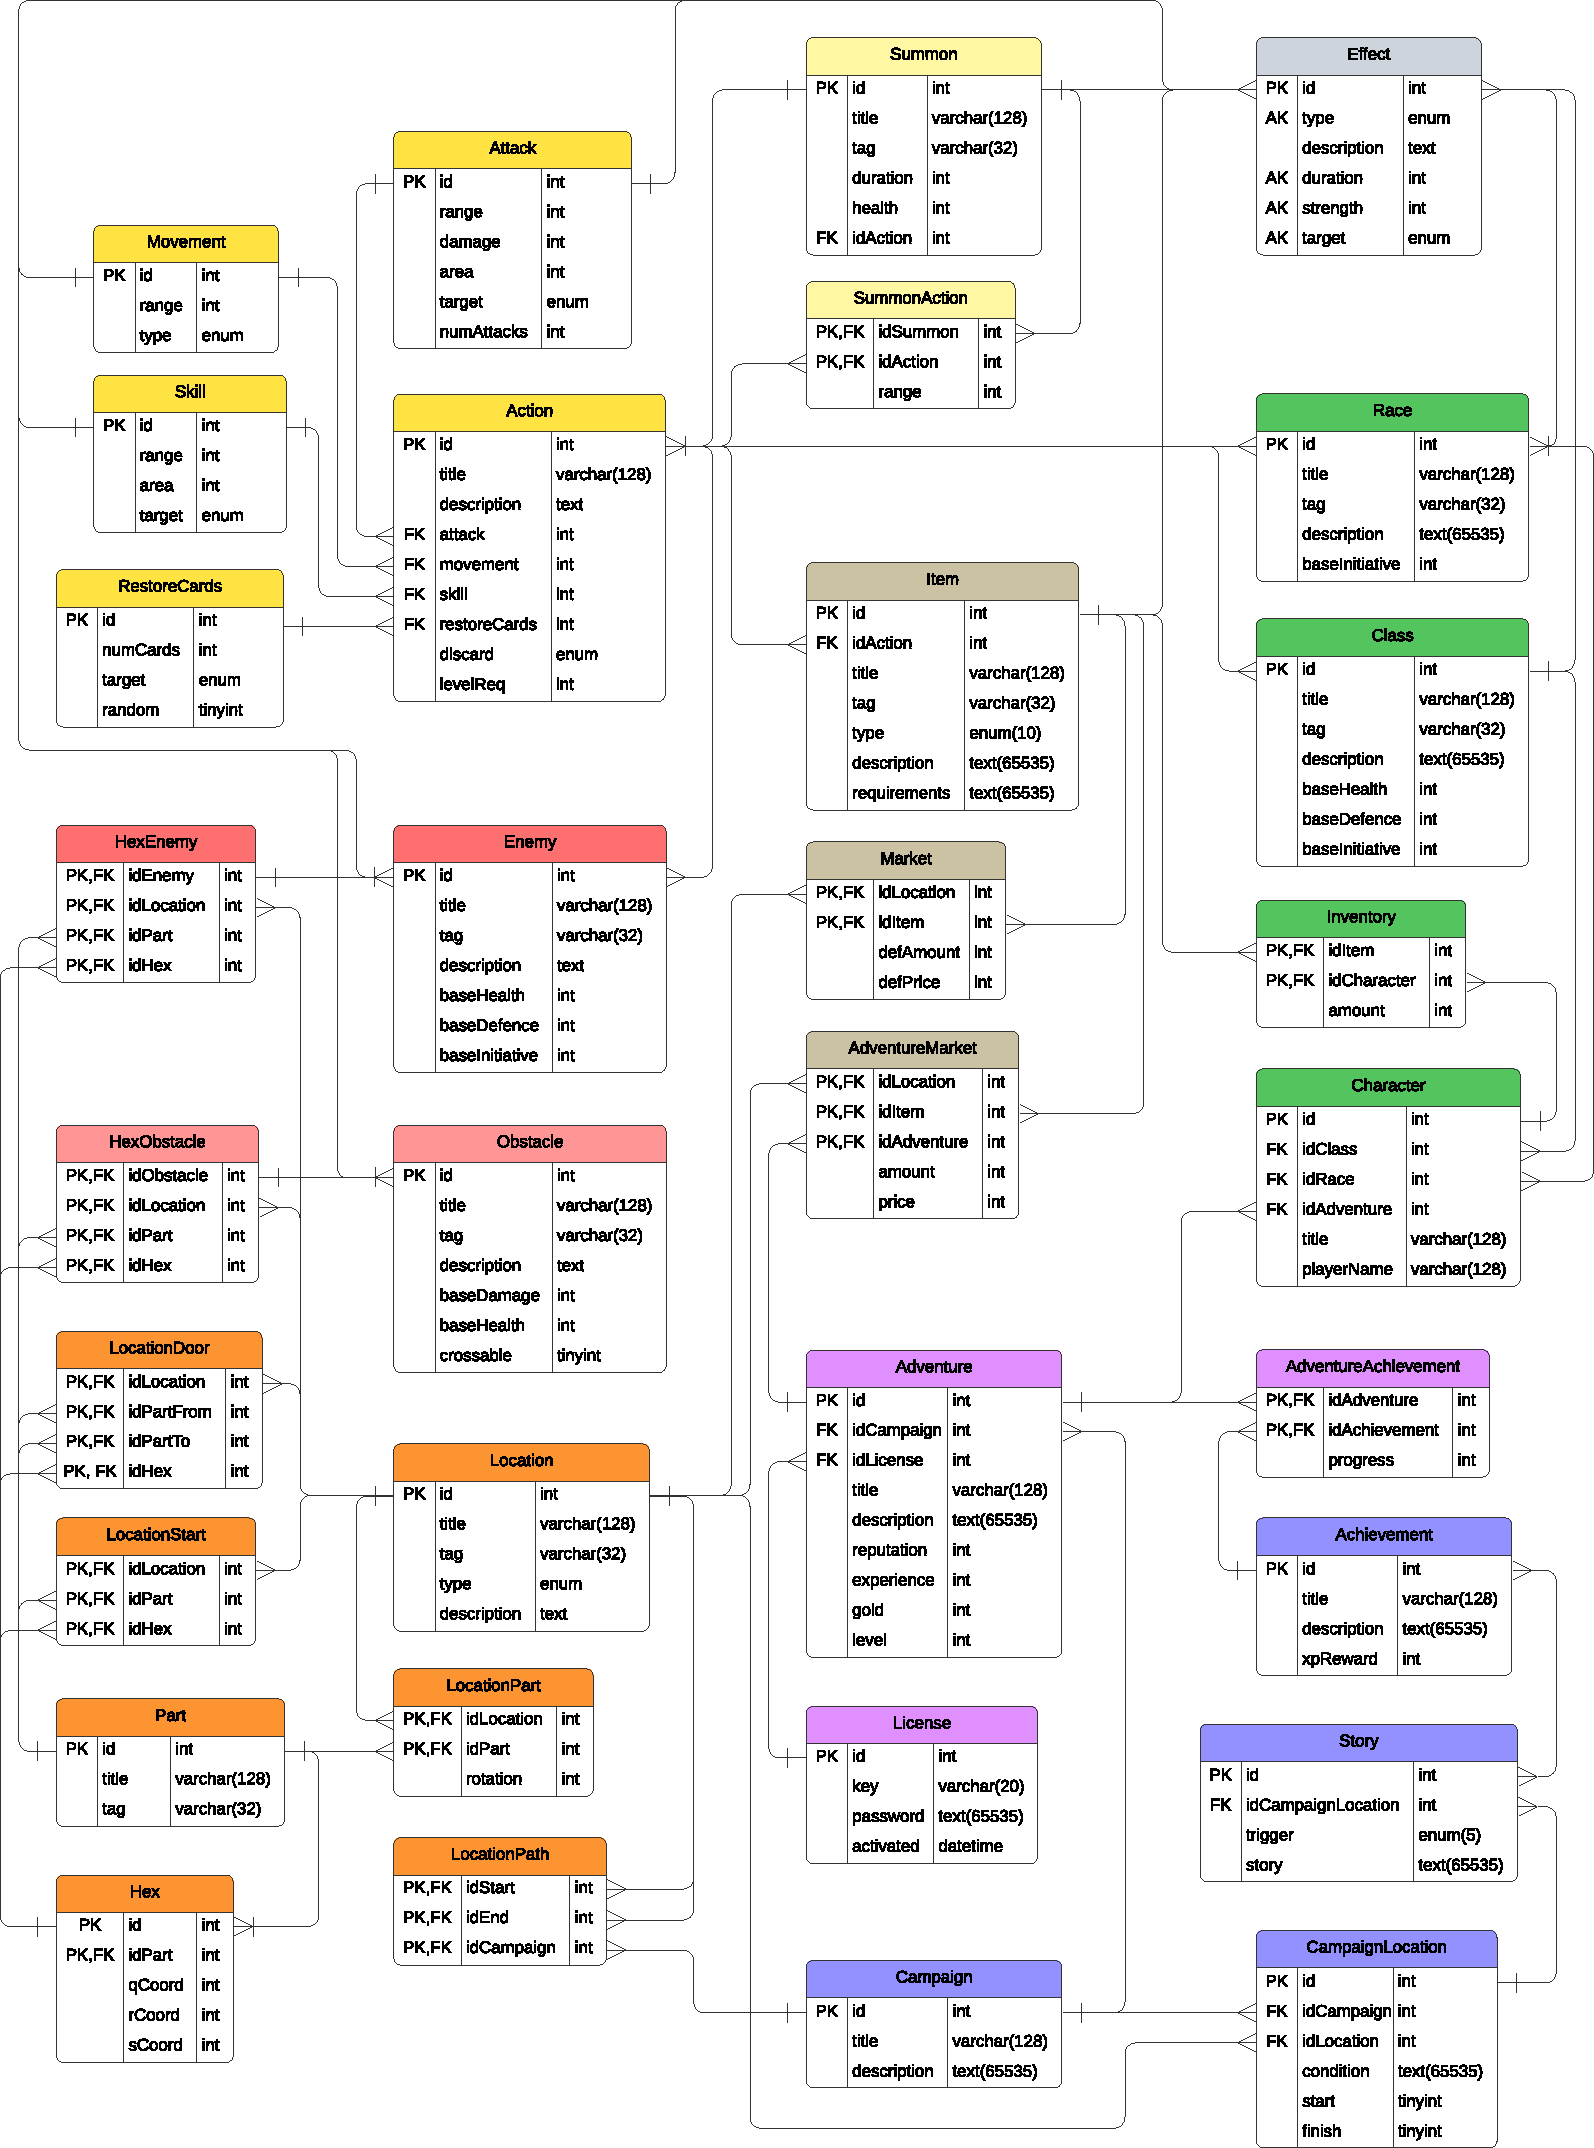
\includegraphics[width=0.96\textwidth]{../../shared/diagrams/dbScheme}
    \caption{Kompletní schéma databáze}
    \label{fig:db_scheme}
\end{figure}

\begin{figure}[H]
    \centering
    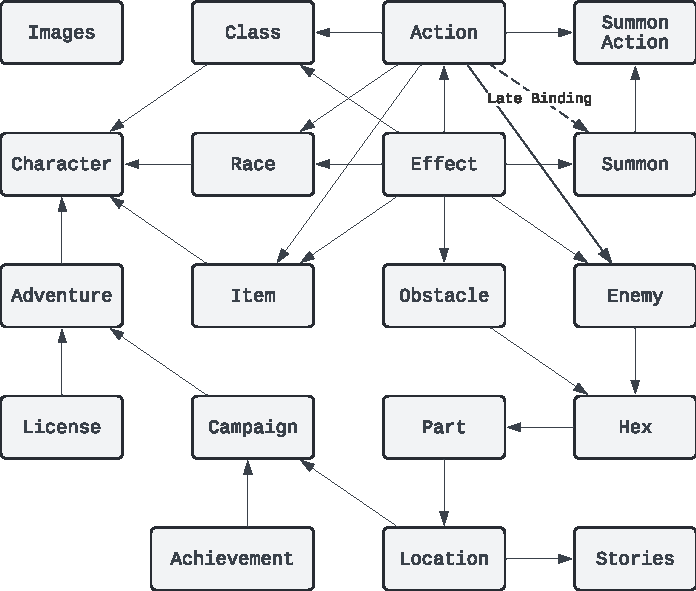
\includegraphics[width=0.7\textwidth]{diagrams/databasePriority}
    \caption{Schéma závislosti tabulek v databázi}
    \label{fig:db_table_priority}
\end{figure}

\begin{table}[H]
    \centering
        \begin{tabular}{l c l}
            \toprule

            \textbf{Název tabulky} & \textbf{Priorita} & \textbf{Závislost} \\
            \midrule

            \textbf{Effect} & 1 & -- \\
            \textbf{Achievement} & 1 & -- \\
            \textbf{Images} & 1 & -- \\
            \textbf{Parts} & 1 & -- \\
            \textbf{Obstacles} & 2 & Effect \\
            \textbf{Summons} & 2 & Effect \\
            \textbf{Enemies} & 3 & Effect, Action \\
            \textbf{Locations} & 3 & Part \\
            \textbf{Races} & 3 & Effect, Action \\
            \textbf{Items} & 3 & Effect, Action \\
            \textbf{Summons (Late Binding)} & 3 & Action \\
            \textbf{Campaigns} & 4 & Location, Achievement \\
            \textbf{Stories} & 4 & Location \\
            \textbf{Adventure} & 5 & License, Campaign \\
            \textbf{Characters} & 6 & Class, Race, Item, Adventure \\

            \bottomrule
        \end{tabular}
    \caption{Tabulka s prioritou dle Diagramu~\ref{fig:db_table_priority}
    \label{tab:db_table_priority}}
\end{table}

\section{Týmová spolupráce}
\label{sec:implementation-collaboration}
Týmová spolupráce ve čtyřčlenném týmu studentů se stává obzvláště komplikovaná v době, kdy je projekt rozdělen do separátních části, které jsou na sobě závislé a je nutná vzájemná komunikace a spolupráce. Jako hlavní a nejvíce důležitou komponentou tohoto projektu se stává API, která slouží pro kompletní komunikaci v rámci projektu. V této sekci se zaměřím na to, jak jsme si rozdělili práci a jaký software jsme k tomu využili.

\subsection{Rozdělení práce}
\label{subsec:implementation-collaboration-distribution}
Rozdělení práce v týmu bylo provedeno tak, že každý člen měl dle zadání přidělenou určitou hlavní část projektu, za kterou byl plně zodpovědný. Každá z těchto částí pak byla následně rozdělena na menší sekce, na kterých se daní členové podíleli buď samostatně, nebo ve spolupráci. Ta je zobrazena v šedém boxu, kde její vnitřní barevné čtverce reprezentují dané členy. Ve výsledném rozdělení práce na Obrázku~\ref{fig:job_distribution} je tak navíc jasně velikostně zobrazena náročnost jednotlivých částí projektu.

\begin{figure}[H]
    \centering
    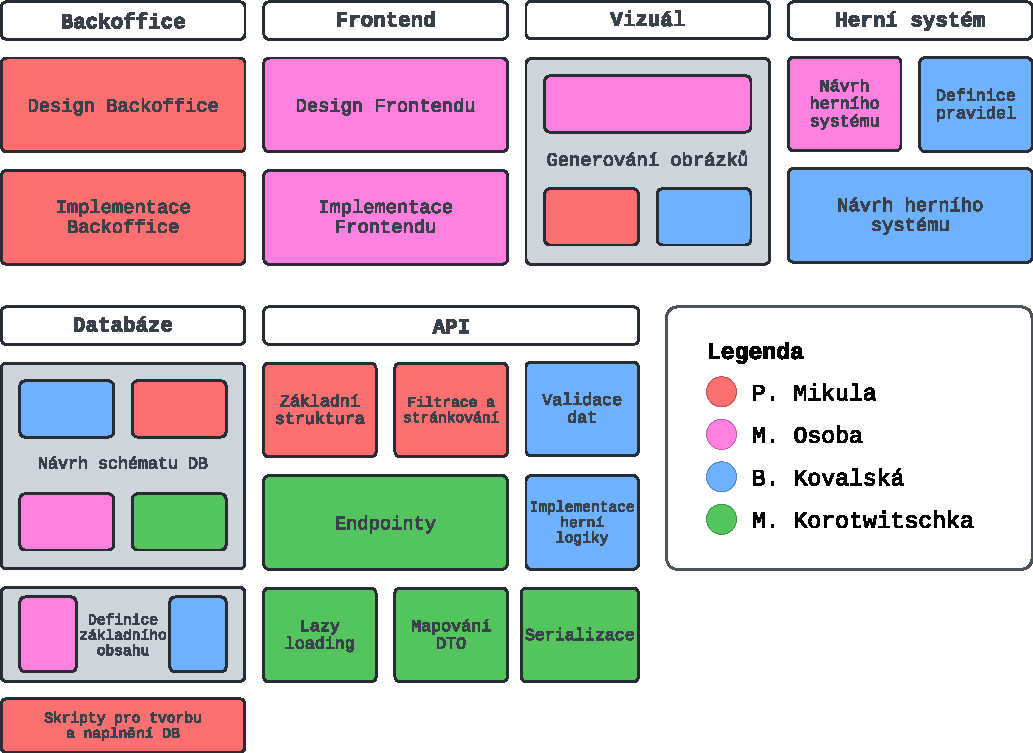
\includegraphics[width=0.95\textwidth]{../../shared/diagrams/blocks}
    \caption{Rozložení práce v týmu}
    \label{fig:job_distribution}
\end{figure}

\subsection{Verzování kódu}
\label{subsec:implementation-collaboration-versioning}
Efektivnost verzování kódu je důležitou součástí každé týmové spolupráce na větším projektu. Pro správu obsahu práce jsme využili nástroj Git pod službou GitHub\footnote{https://github.com/}, který nám umožnil efektivně sledovat změny a udržovat si přehled o vývoji projektu. Využití Gitu bylo zvoleno především pro jeho jednoduchost a znalost všech členů týmu, kteří s ním již měli zkušenosti v minulosti.

\subsubsection*{Větve}
\label{subsubsec:implementation-collaboration-versioning-branches}
V moderních vývojích systému se každá část nebo projekt rozděluje do složitějšího stromu větví. Tento proces je známý pod názvem \textit{Git Worfkflow}, jeho efektivní reprezentaci lze vidět na Obrázku~\ref{fig:git_workflow}. Tento strom se dělí na vícero větví, kde mezi ty hlavní tři patří \textit{live} neboli master, \textit{develop} a \textit{uat} (User Acceptance Testing) známá jako testing branch.

Větev \textit{master} slouží pro produkční verze projektu, které jsou již plně připraveny k nasazení, zatímco větev \textit{develop} slouží pro vývoj nových funkcí případně oprav chyb. Při vývoji nové funkce se pak každá tato aktualizace dostává pomocí tzv. \textit{pull requestu} do větve testovací. V této větvi pak dochází ke konstantnímu testování celého systému a pokud je vše v pořádku, aktualizace se dostávají do produkční větve.

Následně strom obsahuje pod větve vývojové, které se štěpí z větve developu a slouží pro vývoj nových funkcí nebo opravu chyb. Po dokončení a úspěšném testování je tato větev spojena zpět do developu a po vydání nové verze je spojena do masteru.

\subsubsection*{Zkratky}
Tabulka zkratek je zobrazena v Obrázku~\ref{fig:git_workflow}. Nejedná se zde o funkční příkazy softwaru Git, ale o pouhé zkratky pro přehlednější vyobrazení v schématu.

\begin{table}[H]
    \centering
    \resizebox{\textwidth}{!}{%
        \begin{tabular}{l l l}
            \toprule

            \textbf{Příkaz} & \textbf{Zkratka} & \textbf{Význam} \\
            \midrule

            \textbf{git nh} & New Hotfix & Vytvoření větve pro rychlou opravu chyb, která je již v produkci \\
            \textbf{git mh} & Merge Hotfix & Dokončení opravy chyby a spojení větve zpět do masteru \\
            \textbf{git live} & Release & Publikace nové verze a spojení větve do masteru \\
            \textbf{git nb} & New Bugfix & Vytvoření větve pro opravu chyb, která je ve vývoji \\
            \textbf{git mb} & Merge Bugfix & Dokončení vývoje a spojení větve zpět do developu \\
            \textbf{git uat} & User Acceptance Testing & Vytvoření větve pro testování nové verze \\
            \textbf{git nf} & New Feature & Vytvoření větve pro vývoj nové funkce \\
            \textbf{git mf} & Merge Feature & Dokončení vývoje a spojení větve zpět do developu \\

            \bottomrule
        \end{tabular}}
    \caption{Seznam zkratek pro větve v Git Workflow dle Obrázku~\ref{fig:git_workflow}
    \label{tab:git_workflow}}
\end{table}

\begin{figure}[H]
    \centering
    \includegraphics[width=0.9\textwidth]{figures/GitWorkflow}
    \caption{Ukázka správného použití verzovacího systému Git \cite{git_workflow}}
    \label{fig:git_workflow}
\end{figure}

\subsection{Sdílení kódu}
\label{subsec:implementation-collaboration-sharing}
Sdílení kódu není ve vývoji softwaru novinkou, neboť kód ve větším týmu spravuje vícero programátorů. Pro náš účel jsme opět použili systém \textit{GitHub}\footnote{https://github.com/}, kde po založení organizace dostávají všichni členové možnost zapojit se do vývoje. Obrázek~\ref{fig:git_organization} zobrazuje reprezentaci organizace na webové stránce \textit{GitHub}\footnote{https://github.com/Trails-Through-Shadows}, v níž jsou zobrazeny jednotlivé části projektu, jejich krátký popis a jazyk, který v dané části převládá.

\subsection*{Rozdělení částí}
\label{subsec:implementation-collaboration-sharing-parts}
Při zakládání organizace také došlo k zakoupení domény, na kterou následně byly jednotlivé produkční verze nasazeny pomocí dalšího z nástrojů GitHubu a to \textit{GitHub Actions}\footnote{\href{https://github.com/features/actions}{https://github.com/features/actions}}, který slouží pro automatizaci testování a následného nasazení funkční verze na server. Tento systém nám umožnil přehledný a automatický proces spuštění aplikace v praxi.

\noindent
V rámci organizace byly vytvořeny následující části:

\begin{itemize}
    \item TTS-Thesis    -- obsahuje texty diplomové práce od jednotlivých členů týmu se sdílenými materiály, který se nachází pod odkazem \url{https://docs.tts-game.fun/thesis/intro}.
    \item TTS-Database  -- obsahuje skripty pro vytvoření a naplnění databáze základními daty, jejichž schéma je viditelné na Obrázku~\ref{fig:db_scheme} nebo pod odkazem \url{https://db.tts-game.fun}.
    \item TTS-API       -- obsahuje zdrojové kódy API, které slouží pro komunikaci mezi frontendem a backendem. Funkční produkční verze běží pod odkazem \url{https://api.tts-game.fun}.
    \item TTS-Dashboard -- obsahuje zdrojové kódy frontendu, který slouží pro zobrazení dat a správu aplikace. Produkční verze nalezena pod odkazem \url{https://dashboard.tts-game.fun}.
    \item TTS-Frontend  -- obsahuje frontend, který slouží pro interakci s uživatelem. Produkční verze dostupná na \url{https://play.tts-game.fun}.
    \item TTS-Docs      -- obsahuje dokumentaci k projektu která je volně dostupná pod odkazem \url{https://docs.tts-game.fun/data/intro}.
\end{itemize}

\begin{figure}[H]
    \centering
    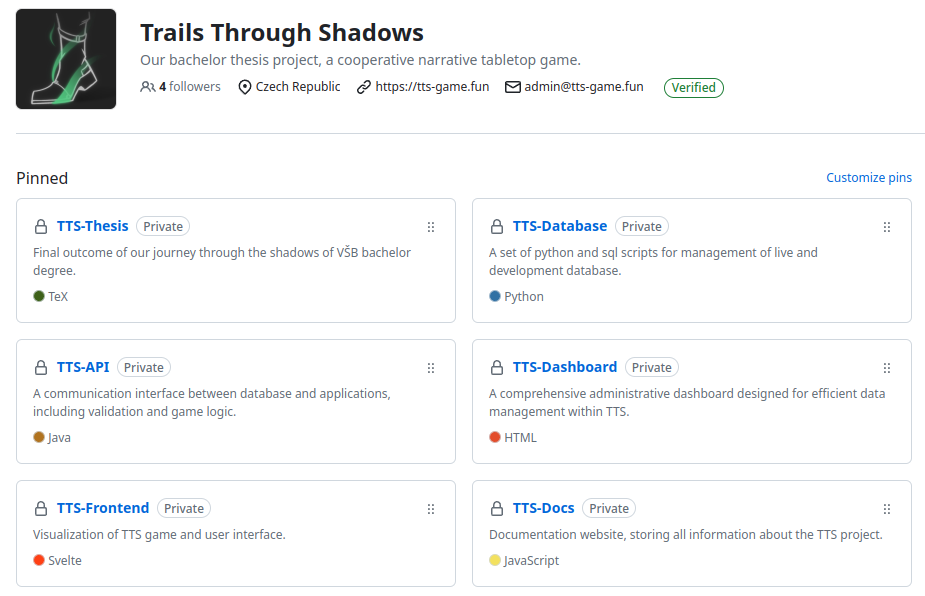
\includegraphics[width=0.9\textwidth]{../../shared/figures/gitOrg}
    \caption{Zobrazení organizace a jejich částí na stránce Github}
    \label{fig:git_organization}
\end{figure}

\subsection{Řešení problémů}
\label{subsec:implementation-collaboration-problems}
Pro řešení problému a chyb v softwaru bylo pro tuto práci využito dalšího z nástrojů webu Github a to konkrétně \textit{Github Issues}\footnote{\href{https://github.com/features/issues}{https://github.com/features/issues}}, který slouží pro ukládání a monitoring problému v projektu. Jako jednu z výhod tento nástroj přináší možnost přiřazení problému danému členovi nebo automatické vytvoření \textit{feature} větve a následného \textit{pull requestu}.

\section{Problémy vývoje}
\label{sec:implementation-problems}
Během vývoje aplikace se vyskytlo mnoho menších a větších problémů, které bylo nutné řešit a následně eliminovat. V této sekci práce se tak zaměřím na ty větší problémy, které přinesly největší výzvu během vývoje.

\subsection*{Hexagonální grid}
\label{subsec:implementation-problems-hexagon}
Během implementace bylo nutné vykreslit hexagonální mapu, která slouží jako základ pro reprezentaci lokace, například jeskyně (z anglického \textit{dungeon}). Tato mapa reprezentuje bojové pole, kde se odehrává herní děj, a je tedy nezbytné správně zaznamenat polohu každého objektu na mapě do databáze, včetně umístění každého hexagonu na plánku, který byl zobrazen.

Při používání hexagonálního rozložení bylo nezbytné načítat z databáze veškeré hexagony, jejich sousedy a vazby, které obsahují s dalšími objekty. Po několika pokusech s klasickými souřadnicemi ve formátu \textit{(x, y)} nám bylo doporučeno přejít na souřadnicový systém osový, známý jako \textit{axial coordinates}, který je reprezentován formátem \textit{(q, r, s)}. Tento systém je používán právě v hexagonálních hrách, protože usnadňuje výpočet vzdálenosti mezi hexagony a identifikaci jejich sousedů pomocí třetí osy.

Pro ověření správnosti souřadnic je možné sečíst všechny souřadnice hexagonu, které by měly dát výsledek 0. Tento výpočet je zobrazen v Rovnici~\ref{eq:axial-coordinates-verification}.
\begin{equation}
    q + r + s = 0\label{eq:axial-coordinates-verification}
\end{equation}

Hexagon jako samotný má možnost mít šest sousedů, které lze vidět na obrázku vedle Rovnice~\ref{eq:hexagon-neighbors}. V případě použití normálního souřadnicového systému by bylo zapotřebí vytvořit složitý algoritmus pro výpočet sousedů, zatímco v případě osových souřadnic stačí ke každému koordinátu přičíst nebo odečíst číslo 1. Výpočet sousedů je zobrazen v Rovnici~\ref{eq:hexagon-neighbors}. \cite{hexagon_grid}

\begin{equation}
    \vcenter{\hbox{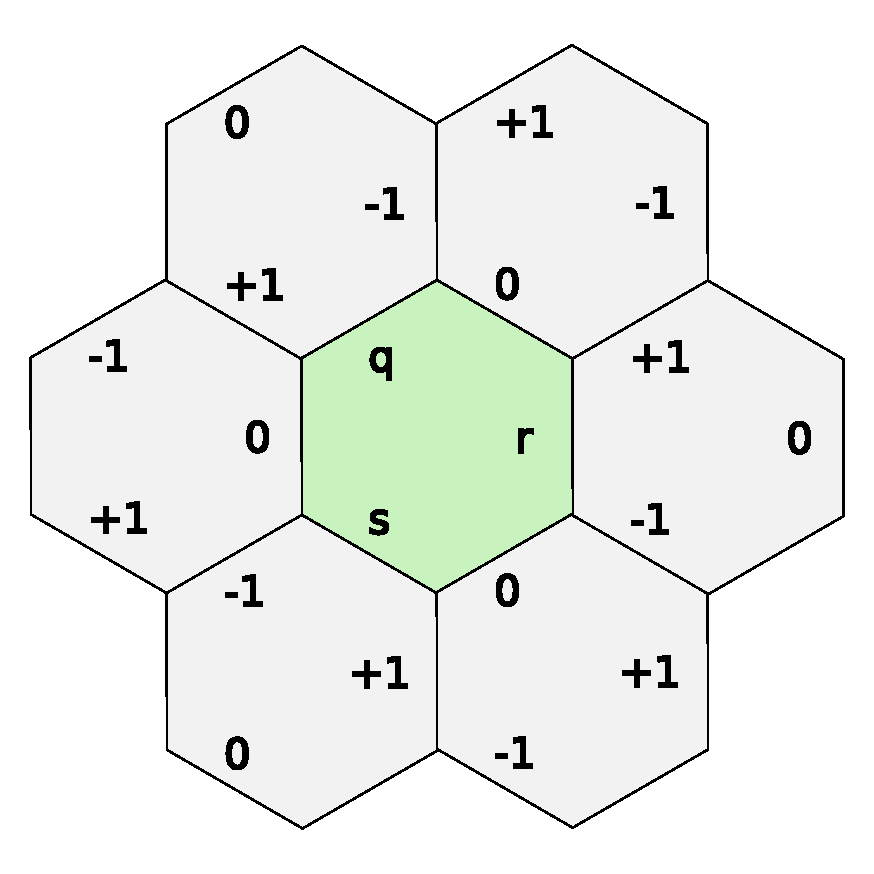
\includegraphics[width=6cm,height=6cm]{diagrams/hexagonNeighbors}}}
    \qquad\qquad
    \begin{aligned}
        \text{Vrchní Levý} & : (q, r - 1, s + 1) \\
        \text{Vrchní Pravý} & : (q + 1, r - 1, s) \\
        \text{Levý} & : (q - 1, r, s + 1) \\
        \text{Pravý} & : (q + 1, r, s - 1) \\
        \text{Dolní Levý} & : (q - 1, r + 1, s) \\
        \text{Dolní Pravý} & : (q, r + 1, s - 1)
    \end{aligned}\label{eq:hexagon-neighbors}
\end{equation}

\subsection*{Časová náročnost}
\label{subsec:implementation-problems-time}
Dalším z problémů, který byl zaviněn špatným návrhem byla časová náročnost aplikace. Vzhledem k tomu, že návrh projektu byl proveden bez zohlednění časové náročnosti, pro dokončení práce bylo zapotřebí vynechat několik funkcí, mezi které patří implementace \textit{summons}, \textit{items}, \textit{achievements} a také správa uživatelských dat, které byly původně plánovány jako součást hry.

Tyto funkcionality jsou v rozhraní označeny jako rozpracované, protože bych se k nim v budoucnu rád vrátil a dokončil jejich implementaci.

\subsection*{Chyba volby frameworku}
\label{subsec:implementation-problems-framework}
Během vývoje rozhraní se postupně nabalovaly problémy, které vybraný framework obsahoval. Jeho volba totiž nebyla dostatečně promyšlená a nebyl zohledněn fakt, že i administrativní rozhraní obsahuje část uživatelskou. Z tohoto důvodu by bylo vhodné zvolit jiný framework, který se více zaobírá frontendem.

V raných fázích vývoje byl zvolen framework Django, který byl ze všech možností nejvíce známý, neboť jsem s ním pracoval v rámci studia. Později v konečném semestru studia jsem vykonal předmět zaměřující se mimo jiné na framework React, který se okamžitě projevil jako lepší varianta pro psaní administrativního rozhraní. Bohužel vzhledem k časové náročnosti a nedostatku zkušeností s frameworkem React, bylo rozhodnuto zůstat u frameworku Django. Jedná se tedy o chybu, která by mohla v případě pokračování vývoje způsobit problémy.

\endinput